\documentclass{article}
\usepackage[UTF8]{ctex}
\usepackage{amsmath,mathtools,geometry,pgfplots,float,mathrsfs,caption,enumerate}
\pgfplotsset{compat=1.15}
\usetikzlibrary{arrows}
\geometry{scale=0.7}

\newcommand\cusong[1]{
	\noindent \rlap{\hspace{0.01em}#1}\rlap{\hspace{0.02em}#1}\rlap{\hspace{0.03em}#1}\rlap{\hspace{0.04em}#1}\rlap{\hspace{0.05em}#1}#1
}

\title{\cusong{每日一题(21.1)}}
\author{\kaishu 李政毅}
\date{2022年6月14日}

\begin{document}
\maketitle
\begin{enumerate}
	\renewcommand{\labelenumi}{\textbf{\theenumi. }}
	\item 设$\triangle ABC$为等边三角形, $P$为$\triangle ABC$ 内任意一点. 过$P$作$PD$, $PE$, $PF$垂直于$BC$, $CA$, $AB$于$D$, $E$, $F$. 求证:
	\[\frac{PD+PE+PF}{AB+BC+CA}=\frac{1}{2\sqrt{3}}.\]
	\rightline{\tiny\kaishu (小学一年级趣味知识竞赛试题)}
	\item 在$\triangle ABC$中, $E$, $F$为$AC$, $AB$中点, $D$为$BC$上任意一点. $P$在$BF$上, 满足$DP\parallel CF$; $Q$在$CE$上, 满足$DQ\parallel CE$. $PQ$交$BE$, $CF$于$R$, $S$. 求证: $PQ=3RS$.\\
	{\small (提示: 梅涅劳斯定理(我想到的较简单的方法).)}
	\begin{figure}[H]
		\flushright
		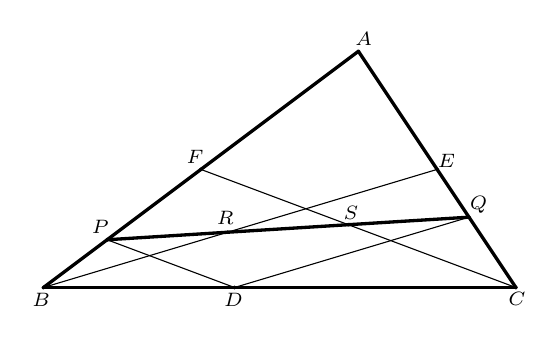
\begin{tikzpicture}[line cap=round,line join=round,>=triangle 45,x=1.0cm,y=1.0cm]
			\clip(-0.2,-0.4) rectangle (6.2,3.3);
			\draw [line width=1.2pt] (4.,3.)-- (0.,0.);
			\draw [line width=1.2pt] (0.,0.)-- (6.,0.);
			\draw [line width=1.2pt] (6.,0.)-- (4.,3.);
			\draw [line width=0.4pt] (0.,0.)-- (5.,1.5);
			\draw [line width=0.4pt] (5.404420156318791,0.8933697655218134)-- (2.4265209379127466,0.);
			\draw [line width=0.4pt] (2.4265209379127466,0.)-- (0.8088403126375822,0.6066302344781866);
			\draw [line width=0.4pt] (6.,0.)-- (2.,1.5);
			\draw [line width=1.2pt] (0.8088403126375822,0.6066302344781866)-- (5.404420156318791,0.8933697655218134);
			\begin{scriptsize}
				\draw [fill=black] (0.,0.) circle (0.5pt);
				\draw[color=black] (-0.027315597952206973,-0.15286251573812404) node {$B$};
				\draw [fill=black] (4.,3.) circle (0.5pt);
				\draw[color=black] (4.067169505172222,3.15903751415915) node {$A$};
				\draw [fill=black] (6.,0.) circle (0.5pt);
				\draw[color=black] (6.014241167361361,-0.1403411545664897) node {$C$};
				\draw [fill=black] (2.4265209379127466,0.) circle (0.5pt);
				\draw[color=black] (2.414349830516489,-0.15912319632394117) node {$D$};
				\draw [fill=black] (5.,1.5) circle (0.5pt);
				\draw[color=black] (5.118963843589507,1.6063887288764962) node {$E$};
				\draw [fill=black] (2.,1.5) circle (0.5pt);
				\draw[color=black] (1.9260167448227499,1.6627348541488507) node {$F$};
				\draw [fill=black] (0.8088403126375822,0.6066302344781866) circle (0.5pt);
				\draw[color=black] (0.7239660723458533,0.7737182109628147) node {$P$};
				\draw [fill=black] (5.404420156318791,0.8933697655218134) circle (0.5pt);
				\draw[color=black] (5.525908081667622,1.0491881567387695) node {$Q$};
				\draw [fill=black] (2.3407002605313183,0.7022100781593956) circle (0.5pt);
				\draw[color=black] (2.307918260557597,0.8801497809217064) node {$R$};
				\draw [fill=black] (3.8725602084250546,0.7977899218406045) circle (0.5pt);
				\draw[color=black] (3.9043918099409756,0.949017267365695) node {$S$};
			\end{scriptsize}
		\end{tikzpicture}
	\end{figure}
	\rightline{\tiny\kaishu (小学一年级趣味知识竞赛试题)}
\end{enumerate}
\newpage
{\large \heiti 附: 梅涅劳斯定理}
\par 如图, $\triangle ABC$的边上有$D$, $E$, $F$三点, 且$D$, $E$, $F$共线. 则:
\[\frac{AF}{FB}\cdot\frac{BD}{DC}\cdot\frac{CE}{EA}=1.\]
\begin{figure}[H]
	\centering
	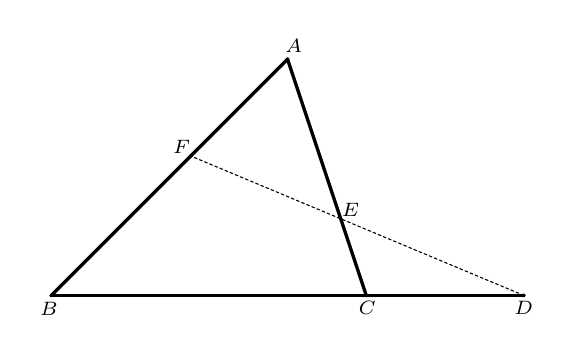
\begin{tikzpicture}[line cap=round,line join=round,>=triangle 45,x=1.0cm,y=1.0cm]
		\clip(-0.3,-0.4) rectangle (6.3,3.4);
		\draw [line width=1.2pt] (3.,3.)-- (0.,0.);
		\draw [line width=1.2pt] (0.,0.)-- (4.,0.);
		\draw [line width=1.2pt] (4.,0.)-- (3.,3.);
		\draw [line width=1.2pt] (4.,0.)-- (6.,0.);
		\draw [line width=0.4pt,dash pattern=on 1pt off 1pt] (6.,0.)-- (1.7704713981362032,1.7704713981362032);
		\begin{scriptsize}
			\draw [fill=black] (0.,0.) circle (0.5pt);
			\draw[color=black] (-0.029291302551187018,-0.16618319856131727) node {$B$};
			\draw [fill=black] (3.,3.) circle (0.5pt);
			\draw[color=black] (3.078222186724025,3.1750813053938822) node {$A$};
			\draw [fill=black] (4.,0.) circle (0.5pt);
			\draw[color=black] (4.013226245444001,-0.15243313887425883) node {$C$};
			\draw [fill=black] (6.,0.) circle (0.5pt);
			\draw[color=black] (6.000109870223947,-0.15243313887425883) node {$D$};
			\draw [fill=black] (1.7704713981362032,1.7704713981362032) circle (0.5pt);
			\draw[color=black] (1.6550910091134745,1.8894507246539183) node {$F$};
			\draw [fill=black] (3.675681838078693,0.9729544857639212) circle (0.5pt);
			\draw[color=black] (3.8001003202945944,1.0919472628045293) node {$E$};
		\end{scriptsize}
	\end{tikzpicture}
\end{figure}
\end{document}